\documentclass[a4paper,12pt]{article}

\usepackage[utf8]{inputenc}
\usepackage[margin=0.7in]{geometry}
\usepackage{lipsum}
\usepackage{tabularx}
\usepackage{caption}
\usepackage{wrapfig}
\usepackage{graphicx}
\usepackage{parskip} % For paragraph indentation and spacing
\usepackage{fontspec}
\usepackage{fontawesome5}
\usepackage[hidelinks]{hyperref}
\usepackage[x11names]{xcolor}
\usepackage[absolute]{textpos}
\usepackage{sectsty} % For section coloring
\usepackage{multicol}

\setmainfont{Garamond}

\newcommand\cvaltcolor{olive}
\definecolor{darkGreen}{HTML}{152614}
\definecolor{teaGreen}{HTML}{dbf4ad}
\newcommand\cvsecondarycolor{darkGreen}
\newcommand\cvsecondarybackgroundcolor{teaGreen}

\graphicspath{ {./images/} }

\hypersetup{
  colorlinks=true,
  allcolors=\cvaltcolor,
}

%% \pagecolor{teaGreen}
\subsectionfont{\color{\cvsecondarycolor}}

\newcommand\cvtitle[2]{\Huge{\bf{#1}} \Huge{#2}}
\newcommand\cvcontact[3] {
  \small {
    \href{mailto:#1}{\faAt \quad #1} \\
    \href{tel:#2}{\faPhone \quad #2} \\
    {\href{https://www.linkedin.com/in/#3/}{\faLinkedin \quad linkedin}}
  }
}

\newcommand\cvhrule{{\color{gray}\hrule}}
\newcommand\cveducation[4]{

  \normalfont\bf{#1, #2}

  \normalfont\small{#3 (#4)}
}

\newcommand\cvte[2]{\footnotesize{\textbf{#1}} ~$\cdots$~ & \footnotesize{#2}}

\newcommand\cvsubsection[3]{\subsection*{#1 \quad \small{(#2 - #3)}}}
\newcommand\cvprojectentry[5]{
  \subsubsection*{#1}
  
  \vspace{-7pt}
  
  \it{Domain: #2}\normalfont{} \quad (#3 - #4)
  
}

\begin{document}

\begin{minipage}[b]{.69\linewidth}
  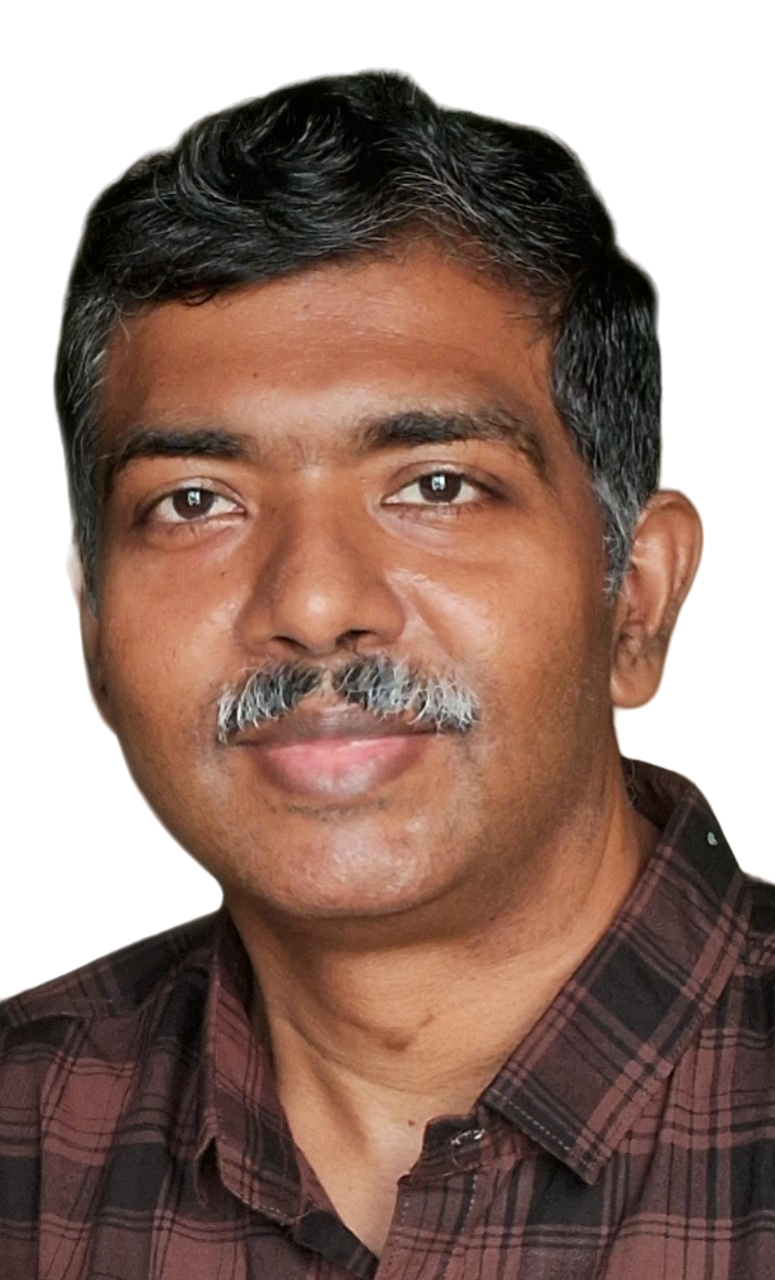
\includegraphics[height=3\baselineskip]{me}
  \cvtitle{Shoban}{Jayaraj}
\end{minipage}
\begin{minipage}[b]{.3\linewidth}
  \cvcontact{shobanj@hcltech.com}{+91-98401-46057}{shobanj}
\end{minipage}

\cvhrule


\includegraphics[height=1.5\baselineskip]{agile}

\includegraphics[height=1.5\baselineskip]{pmp}

\begin{wraptable}{r}{6cm}
  \caption*{Timeline}
  \begin{tabular}{l|p{4cm}}
    \hline
    \cvte{2024}{Drove and achieved 150\% Value add and SixSigma initiative targets} \par \textbf{Patent Granted} - \href{https://patents.justia.com/patent/20240281181}{Using LIDAR To Define Printable Area For Document Printing} \\
    \cvte{2023}{Developed \& showcased a hands free AR / AI based guidance system \par Key member of patent review board and improved selection rate by 70\% } \\
    \cvte{2022}{Devloped R / Python based  Knowledge Management Capability assessment and analysis tool - recognized as a SixSigma project} \\
    \cvte{2021}{Prototyped 3D / AR app - enabled winning an AR application dev contract} \\
    \cvte{2020}{\textbf{CMMI Appraisal Team Member (ATM)} - Took part in CMMI assessment and achieved Level 5 for group} \\
    \cvte{2017}{Poster presentation for TUG - `Application of Big Data Analytics in the ATE domain'} \\
    \cvte{2014}{SME for OOAD UML, Design Patterns, Requirements Management - Trained over 500 members (>250 hrs.) since 2008} \\
    \cvte{2011}{Gained confidence with client by building a UI mockup of the NUI application using Qt/QML over the weekend} \\
    \cvte{2010}{PoC on production printer simulator frontend using Qt/C++ which kickstarted taking up the work} \\
    \cvte{2001}{ezTest prototyped as a personal initiative and became a line of business} \\
    \cvte{1998}{Developed a proxy server for shared internet browsing using Java adopted within org} \\
    \cvte{1997}{Implemented a sliding window content renderer for content of arbitary length} \\
    \hline
  \end{tabular}
\end{wraptable}

{
Have been with the IT industry since June '95 with over twenty nine years
in architecting and managing multiple projects and functions in
domains like printing, semiconductor, telecom, automation, industrial,
and workflow.

\section*{Professional Experience}
  
\cvsubsection{HCL Technologies, Chennai}{Dec 2002}{Till date}

Extensively managed programs and technically contributed on the Office
Automation (Office \& Production Devices), Semiconductor (ATEs, Ball
bonders) and Industrial (Frequency Convertors) domains.

\cvprojectentry{Software Development Support}{Semiconductors}{Jan 2024}{Till date}

Group manager managing over 110 members placed at multiple locations
covering QA and SW development for multiple divisions spanning India
(Chennai, Bengaluru, Mumbai, Pune), US and Canada. Have been
responsible for handling the operational aspects of running the
project covering forecast, billing, fulfillment and customer connect.

Streamlined the recruitment process and \textbf{improved selection rate of
candidates by 3 times}.

\cvprojectentry{Digital Software Solutions}{Office Automation}{Jun 2017}{Dec 2023}

Served as the lead for tracks spanning a total of 45 – 65 members
covering development, sustenance and enhancement of printer drivers,
content management system, logs aquisition \& analysis, \textbf{LIDAR
  based AI model training and inference, AR / VR solution} that used
object and state detection, enterprise / clould based print solutions,
enhancements of a public print kiosk, a playstore equivalent for
printers and associated QA activities.

Front-ended the Six sigma and value added initiative for the account
by tracking targets and \textbf{achieved over 150\% of
  targets}. Encouraged and filtered ideas for patent filing and
\textbf{improved the selection ratio by 70\%} (of which I was the
primary applicant for 3 ideas). In addition, I also guided teams on
evaluating new concepts on emerging technologies such as AI / ML, AR
(Hands free AR, Synthetic image generation), NLP etc.,

\cvprojectentry{ATE Instruments Program}{Semiconductors / ATE}{Jun 2017}{Dec 2018}

Served as the group manager for the software design and development of
components covering AC, DC, RF instruments and supported the team
technically as well as taking care of customer connect, commercials as
well as team management.
  
Started as a team of 4 members working for a single instrument, and
grew this to ~17 members spanning six different instrument and support
projects.

We also started the \textbf{`Instrument Incubation Program'} to scale
up both new joiners and lateral hires to enable instrument development
quicker both in terms of knowledge and enabling support tools.


}

%% \begin{multicols}{2}

\cvprojectentry{64 bit Migration}{Semiconductors / ATE}{Feb 2016}{Jun 2017}

Served as the program manager interacting with the different groups at
the client side to migrate the existing ATE SW application (12M LOC)
from 32 bit to 64 bit to bridge over the 4GB RAM limit.

Supported in porting the software from obsolete technology, evaluated
3rd party components and recommended replacements, conducted
performance evaluation and implemented optimizations while running in
the 64 bit environment, validated all features against the
requirements and ensured conformance to both the 32 bit and 64 bit
environment and support end-user issues during alpha and beta testing
and final release.
 
The program consisted of over 20 members from the software team
interacting with equal number of engineers from the client
organization and SV of similar strength located in three different
geographical locations and time zones. Was responsible for
coordination, tracking of the milestones and progress, identifying and
evaluating risks, productivity measurements and actions, reporting to
different levels of sr. management on the progress and challenges. We
had completed the program successfully 2 weeks ahead of schedule. This
was recognized and \textbf{awarded as a best project executed at this
scale} within the group.

\cvprojectentry{PCSW for configuration \& commissioning}{Industrial / Power Electronics}{Aug 2011}{Feb 2015}

Served as the architect for designing the PC Software framework, built
to be extensible and portable to help the client to adapt to their
various products. The framework allowed for a
service-oriented-architecture with heavy emphasis on \textbf{Natural
  UI (NUI), scalability and robustness}. One realization of the
framework which we designed was to manage motor control devices.
 
Started as a team of 4 members when the requirements were analyzed and
grew to ~40 members from different functions (Testing, automation,
UxD) collaborating using Agile Scrum. Initially functioned as a
technical manager / architect and as the team grew, primarily focused
on the technical aspects of the project.

\cvprojectentry{Production Print and Office Simulator}{Office Automation}{Apr 2009}{Jul 2011}
 
Responsible for developing projects support applications to improve
the efficienc of the QA department (man power, cost, time
reduction). This included developing simulators (for Production,
Office Printers), test automation framework (to test MIB, WebServices
capabilities of the printer) using C++, Qt on Windows and porting
Windows based simulators to Linux.
 
We showed an \textbf{improvement of 17\% over manual testing process} and
increased test coverage to 14.7 times of original.
 
The program consisted of multiple teams / projects totaling strength
of 18 to 8 members working off India and Japan. I am responsible for
customer connect, financials and overall team management (estimation,
tracking, performance evaluation, corrective actions, improvements
etc).
 
\cvprojectentry{Digital Development Support}{Semiconductors / ATE}{Jan 2009}{Mar 2009}
 
Providing development and sustenance support for High Speed Memory
testing capability scheduled for the release of the latest version of
ATE.
 
Was responsible for a team of 7 members, managing the projects and
serving as the client interface for the project.
 
\cvprojectentry{Checkers Maintenance}{Semiconductors / ATE}{Feb 2008}{Dec 2008}

The Test Development Engineering (TDE) Indian team is responsible for
the maintenance programs for the different lines of ATEs, as well as
developing new test programs and tools for DC and AC instruments

The team has been able to perform well above the stipulated
productivity goals in sustaining the software and had constantly
improved the productivity year on year.
 
My responsibility is to manage the team of 11 - 8 members, maintain
customer connect, handle contractual activities like generating SOWs,
billing, monitor the performance of the team and suggest improvement
initiatives.
 
\cvprojectentry{Application Shmoo}{Semiconductors / ATE}{Jan 2007}{Nov 2008}

Shmoo plots are graphical charts that display the response of
electrical components or systems by varying a range of conditions and
inputs like voltage, amplitude, current etc. This is used to observe
the operating ranges of a device.
 
Was responsible for managing a team of 2 engineers to implement the
plotting capability. We are responsible for designing, coding, testing
and verification of the various generations of the application.
 
\cvprojectentry{Analog Tools Program}{Semiconductors / ATE}{Mar 2006}{Nov 2008}

This program involved the team to provide development support and
sustenance of all analog tools of the ATEs. This involved me and my
team to develop a code generator that tracks user's changes to debug
displays for over 32 instruments, signals / PSet (parameter set)
editor, the Characterization Editor that allowed the user to
graphically create characterization schematics to test a device,
execute the tests and visualize them as a `Shmoo' plot.

The Tester State Service which provide parametric enumeration support
of instrument capabilities which can be queried programmatically. It
also provided support for a wizard to generate scaffolding code in
DotNet to enable parametric support for new instruments.
 
My responsibility was to manage the specified programs with the team
varying from 3 to 12 engineers, serving as the single point of contact
to the customer, collaborating with other functions like software
verification and test team, automation team and the process compliance
team. I had also contributed technically in most of the projects.
 
Awarded 5/5 on customer satisfaction and awarded the HCL GoldLine
award for successful completion of the program. Was appreciated by the
client on my ideas and initiatives of creating reusable components,
thus saving time in their future projects
 
\cvprojectentry{HVD, HDVS and Microwave – Autotest Development and
  Ownership}{Semiconductors / ATE}{September 2004}{September 2006}

The High Voltage Digital, High Density Voltage Source and Microwave
are instruments that plug into the automated test equipments designed
to test devices. This project involved us to own all auto-tests (75+)
which include development of new auto-tests using VBA, Perl, C++/COM
and CPPUnit to test the features of the instrument, extending existing
tests for cover new features and monitoring and resolving auto-test
failures. We had also resolved a few defects with the instruments sw.
 
My responsibility within the team is to plan, schedule and manage the
team of 4 for development and sustenance of auto-tests. In addition
to management, I am also responsible for process compliance and
contributing to the technical aspects of development.
 
\cvprojectentry{GUI Decoupling}{Semiconductors / Wire Bonders}{October 2003}{September 2004}

This project refactors the wire bonder tool by decoupling the domain
specific workflow from the UI using the MVC approach. The goal of the
project is to improve developer productivity, enable split development
teams to work on the GUI and the application and provide a migration
path to move to Windows XPE and .NET from vxWorks and X/Motif. With
major feature enhancements happening in parallel, we chose to use an
iterative approach that incorporates incremental features.
 
My role in this project was to help recommend the architecture,
estimate, plan, architect and collaborate with the various teams in
realizing the design. I also managed a team of four to complete the
communication framework using C++, Visual C++, vxWorks.
 
\cvprojectentry{Distributed Material Handling System}{Semiconductors / Wire Bonders}{January 2003}{October 2003}

A new feature request for the wire bonder suite of tools that aims to
move away from the proprietary VME bus to off-the-shelf PC based
systems via Ethernet. It allows multiple distributed modules that can
be connected to the bonder tool. Each module is responsible for
controlling a specific set of devices like sensors, steppers and
solenoids. The project also implemented a custom distributed shared
memory component to allow the components to talk with each other.
 
The project was developed using vxWorks on the x86 platform with the
target being a stepper controller running on the Blackfin series of
DSP processors by Analog devices. The stepper board was connected to
the sensor and solenoids via a SPI bus. The project involved
implementing a messaging layer between the host and the target in C++
and a distributed shared memory component that was used by the host
and the target to send stepper commands.
 
Was responsible for architecting the host part of the
system. Initially, the messaging layer was built on VC++ using POSIX
and was later migrated to vxWorks. I managed a team of 4 members to
implement the host part of the software. I was also responsible for
providing on-site training and transition to the members of the
Singapore division

\cvsubsection{Think Business Networks, Coimbatore}{Aug 1997}{Dec 2002}

\cvprojectentry{Digital Nervous System}{Process Workflow}{September 2002}{December 2002}
 
Managed the DNS project, a workflow automation framework that allows
IT related processes to be automated. It aims at reducing the
productivity dip that is caused by following the process manually by
handholding the users on what needs to be done and how. Users can
interactively model processes via activity diagrams, deploy them for
instantiation, map the processes to the various KPAs defined by SEI
CMM (for internal assessment), extract quality metrics etc.
 
My responsibilities were to manage a team of eight members and
incorporate functionalities like CVS support for document archival,
conditional branching and joining of activities within processes etc.
 
DNS was implemented on the .NET platform. 
 
\cvprojectentry{Test Automation Layer}{Test Automation}{August 2002}{December 2002}

Functioned as an architect to design and validate the Test Automation
Layer (TAL) that allowed producing faster automation solutions by
providing functional automation management and deployment tools on top
of existing automation frameworks. TAL employs various test automation
methodologies like CSDDT (Continuous Synchronized Data Driven
Testing), Action / keyword driven testing to provide effective test
automation solutions.
 
\cvprojectentry{Real-time Fault Receiver}{Telecom / Networking}{Mar 2002}{July 2002}

Designed the system and managed a team of 4 for the project, a
component add-on to our product, `Think EMS' to provide the capability
to minimize SNMP based trap loss by providing a real-time solution
using RTJ specs.
 
This highly configurable system functions as a real-time component
running on TimeSys Linux/GPL with Real-time Java extensions to capture
UDP based SNMP traps and relay them back to the EMS for event
correlation and consolidation. The RFR implements its own high
performance customized persistence engine and provides a \textbf{20x
performance boost} in handling SNMP TRAPS compared to the current EMS
implementation.
 
\cvprojectentry{EzTest}{Internet / Web}{July 2001}{September 2002}
 
Was responsible for the architecture and management of the EzTest
project, a part of the Enterprise / University Information Portal
project (E/UIP). EzTest features automated evaluation of candidates on
selected skillsets aiding in recruitment and training
assessment. EzTest used open-sourced software to reduce the cost of
the product.
 
The assessment engine was marketed towards the educational, corporate
and IT enabled services (call centers) segments. Incidentally, the
assessment engine was started by myself as a personal initiative to
help us with our recruitment efforts and was eventually adopted by the
organization. The product was completed with a team of three members.
 
\cvprojectentry{Nuera EMS}{Telecom / Networking}{June 2000}{July 2001}

Was one of the key members involved in the design and development of
an EMS for managing and monitoring Remote Digital Terminals (RDT)
manufactured by Nuera Communication Inc, CA, USA, for their customers
AT\&T. The EMS was designed to manage Fault, Configuration, Performance
and Security (FCAPS) for the system. The RDT was responsible for
enabling IP based voice and data communication within cable TV
networks and interfaces with the external PSTN.
 
Was responsible for the design and managed a team of three to
implement the Fault, Performance and Diagnostics servers for the
system. The servers were based on a pluggable architecture supporting
SNMP southbound and with northbound capabilities to talk to
higher-level managers (like HP OpenView) via SNMP, RMI or e-mail.
 
\cvprojectentry{zGenie}{Internet / Web}{October 1999}{October 2000}

Zgenie is a web community based information sharing tool that brings
content to your desktop rather than wade through millions of
non-relevant information available in the web.
 
Was one of the key architects of the system and managed the client
side implementation of the application with a team of four. The client
side implementation consisted of building COM based plug-in to
Internet Explorer, a lightweight proxy server and a binary
interception engine that allows the users to `Alt+Click' on any text
in any GUI based application and use it as a basis to pull information
off the web. The application also supported the capability to update
itself over the web. The product entered beta with 300+ users using
the application. The product was developed with Microsoft Visual C++
6, with MFC and COM.
 
The application suite was used to power our knowledge management tool
`ezInfo'.
 
\cvprojectentry{WorldStreet Sales}{Securities / Financial}{August 1998}{September 1999}

 
WorldStreet Sales is a financial portal for the securities industry,
capable of consolidating external information like stock quotes, news
feeds, research articles from various sources like IDC, Reuters in
real-time, there by allowing the sales team to provide timely advice to
their clients.
 
My job, as a consultant was to analyze the performance of the system,
identify the shortcomings and overcome the performance issues with
better solutions. This involved developing solutions that required
parallel generation of presentation data for portlets, dynamic caches
to manage real-time quotes and database optimizations.
 
Was responsible for bringing back two projects to be developed
offshore, one being a chart server capable of plotting financial
charts using pricing information obtained from data-feeds maintained
by Reuters and IDC. The other is responsible for uploading external
IDC data-feeds into our database.
 
These projects made extensive usage of Java, RMI, JNI, and JDBC to
achieve its goals.
 
\cvprojectentry{NetExpress}{Telecom / Networking}{August 1997}{August 1998}

NetExpress is a 3-tired distributed system on Windows NT, for the
management of complex services on Nortel’s DMS 100 switches. Basically
the system is responsible for service provisioning (Service Management
System) in the DMS 100 switches and also acts as Operations Support
Systems for the service providers. The system consists of thin clients
spread across a WAN, being serviced by our set of server applications
running on NT server with a backend ORACLE database. This system was
developed entirely in Visual C++ involving rule based, network
modeling and limited object database implementation.
 
Ceon (formally known as FirstTel systems) developed NetExpress for
some of the largest Telcos in the world (Telstra, British Telecom and
etc.).
 
Developed ASUBS (Automatic Service Unit Billing System), a billing
system for the features (around 190 features) provided to customers in
the DMS 100 switch. There was no proper system to produce the billing
for the DMS 100 switches and this is the very first system that
generated accurate feature based billing for DMS 100 switches. ASUBS
is a rule-based system that features capabilities to add new billing
requirements and modify the existing rule without changing the
application.
 
Was also responsible for managing a team of 7 for a feature point
release of NetExpress.

\cvsubsection{L-Cube Innovative Solutions, Chennai}{Jun 1995}{Aug 1997}

\cvprojectentry{Electronic Service Manual}{Document Publishing}{Jun 1995}{Aug 1997}
 
The Electronic Service Manual (ESM) helps in providing quick access of
digitized documents to service personnels in troubleshooting complex
machineries. It featured network decision trees to aid the personnel
in zeroing on the problem, dynamic forms to report problems, an
internal scripting framework, with support for rendering various types
of documents like RTF, WordPerfect Documents, SGML and HTML. The ESM
works as a standalone application and is also capable of collaborating
with other users over the network. The latest incarnation was capable
of generating Internet ready manuals dynamically for access over the
web. ESM was developed using C++.
 
I functioned as a software engineer, responsible for implementing a
display renderer capable of rendering complex documents with supports
for tables, columns etc,. Was also responsible for developing the
web-rendering engine that exports regular word processing documents as
HTML to be accessible over the net.
 
I was also responsible for building the entire automated test
framework, based on MS Test, an early version of Rational Visual Test.

%% \end{multicols}

\section*{Education}

\cveducation{M.S.}{Software Systems}{BITS Pilani}{CGPA 7.94}
\cveducation{B.E.}{Computer Science}{Barathiar University}{74.77\%}

\section*{Other Achievements}

\begin{itemize}
  \item{\bf{HCL Technologies}}
    
    \begin{itemize}
      \setlength\itemsep{-0.5em}

    \item Published a papers on \textbf{`Big data analytics'},
      \textbf{`Machine Learning'} for the internal newsletters, paper
      presentation contest

    \item Created proof of concept application on auto-test
      regression analysis using the ELK (Elasticsearch, Logstash and
      Kibana) stack which led to the focus of extending the same
      within the group for different projects for analysis.

    \item Best project award (4), Goldline award (2) for successful
      execution and completion of projects.
      
    \item Took up various additional roles
      \begin{itemize}
      \setlength\itemsep{-0.5em}
        
      \item Served as \textbf{SKO (Senior Knowledge Officer)} for a
        semi group that I was a part of, promoting Knowledge
        Management Practices by encouraging team to share knowledge to
        our central repository.

      \item \textbf{CMMI Appraisal Team Member} covering
        \textbf{`Delivery \& Managing Services'} Capability area -
        Practice Area: Service Delivery Management \& Strategic
        Service Management for level 5 certification.

      \item \textbf{Editor \& Publisher} for our quarterly Semi
        newsletter distributed to both HCL and customer.
        
      \item \textbf{Six Sigma Semi SPOC} to monitor and drive the
        achievements of our yearly targets for 3 years and had
        exceeded the targets.

      \item \textbf{Patent Reviewer} to streamline and be the first
        line of reviwing the parent applications by the team and
        guiding them to represent their ideas better. Improved
        selection rate next level by 70\%

      \end{itemize}
      
    \end{itemize}

  \item{\textbf{Think Business Networks}}

    \begin{itemize}
      
      \setlength\itemsep{-0.5em}
      
      \item Was part of the SEI CMM internal audit team 

      \item Served as a member of the Quality Improvement Team 

      \item Responsible for `Open Source Software' awareness which 
        lead the organization to use both open source software as well
        as to contribute to the movement

      \item Served as the CTO, conducted many technology based team
        activities within the organization to create awareness of KM
        practices, reusability etc.

      \item Developed, as a personal initiative, EzTest an automated
        testing system to help us with recruitment activities. EzTest
        was adopted by the organization and was commercialized,
        targeting all universities, recruitment agencies, ITeS
        industries, training institutes and schools. EzTest was
        awarded the Quality Improvement Team's best corrective action
        project for 2001
        
    \end{itemize}
\end{itemize}

\section*{Patents \& Publications}

\begin{itemize}
  \setlength\itemsep{-0.5em}

\item
  \textbf{Patent Granted} -
  \href{https://patents.justia.com/patent/20240281181}{Using LIDAR To
    Define Printable Area For Document Printing.}
  
\item
  \textbf{Patent Pending} -
  \href{https://patents.google.com/patent/US20230289515A1}{Methods
    and systems for adding annotations from a printed version of a
    document to a digital version of the document}

\item \textbf{Patent Published} -
  \href{https://patents.google.com/patent/US20190294385A1}{Method and
    system for arranging and printing pages according to search
    criteria}

\item Article on \textbf{`Database Abstraction using PHP'}, a web scripting
  language published in \textbf{Developer IQ, September 2002 edition}.

\item Article on \textbf{`Static Generation of Charts for Web Servers
  on Linux'} – Published in the Linux supplement of
  \textbf{Developer IQ Feb 2002 issue}.

\end{itemize}


\section*{Certifications \& Courses}

\begin{itemize}
  
  \setlength\itemsep{-0.5em}

\item \href{https://partner.cloudskillsboost.google/public_profiles/c3662c2a-8b10-4480-9922-dc384a446a1d}{Generative AI Fundamentals (Google Cloud, 2023)}
  
\item
  \href{https://www.coursera.org/account/accomplishments/specialization/Y9XD9ZQ3EGG2}{Deep Learning Specialization (DeepLearning.AI, 2018)}
  
\item
  \href{https://www.coursera.org/account/accomplishments/verify/2YVCNYET6XSL}{Machine Learning (Stanford University, 2018)}

\item BEC (Business English Certified) Level 2 (University of Cambridge, 2000)
  
\item Sun Certified Java 2 Programmer (Sun Microsystems, 1999)
  
\end{itemize}

\section*{Hobbies}

\centering{

  \href{https://www.flickr.com/photos/shobanjayaraj/}{\faFlickr} Photography |
  \href{https://shoban.itch.io/}{\faItchIo} Game Jams |
  \href{https://www.goodreads.com/user/show/54087481-shoban-jayaraj}{\faGoodreads} Reading |
  \href{https://github.com/shobanj}{\faGithub} Productivity App Development |
  \href{https://shobanj.wordpress.com/}{\faWordpress} Blogging

}

\end{document}
